\chapter{State of the art} % Main chapter title
\label{StateOfTheArt}

\section{Volume rendering algorithms}

The fundamental volume visualization algorithms described
below fall into two main categories: 

\begin{itemize}

\item Direct volume rendering (DVR) algorithms: they include approaches such as ray-casting, texture mapping, splatting, and V-buffer rendering. Splatting and V-buffer are also called projection methods. These these methods are characterized by mapping elements directly into screen space without using geometric primitives as an intermediate representation.

\item Surface-fitting (SF) algorithms : they are also called isosurfacing or feature-extraction. These algorithms consist in fitting surface primitives such as
polygons or patches to constant-value contour surfaces in volumetric datasets. The surface primitives used are most of the time planar.

\end{itemize}

DVR methods are especially appropriate for creating images from datasets containing amorphous features like clouds, fluids, and gases. One disadvantage of using DVR methods
is that the entire dataset must be traversed each time an image is
rendered. A low resolution pass or random sampling of the data is
sometimes used to create low-quality images quickly for parameter
checking. The process of successively increasing the resolution
and quality of a DVR image over time is called progressive
refinement.

 The user begins by choosing a threshold value
and then geometric primitives are automatically fit to the high-contrast
contours in the volume that match the threshold. Cells
whose comer-values are all above the chosen threshold (cell is
inside) or all below the threshold (cell is outside) are discarded and
have no effect on the final image. Showing just the cells falling on
the threshold is sometimes useful, but can be a problem. Another
consideration is the huge number of surface primitives generated
for large volumetric datasets. 


Many steps in the volume visualization process are common to
volume visualization algorithms.  Most of the fundamental volume
visualization algorithms include only a subset of the steps listed
here.
The initial step in every procedure is data acquisition. The next
common step is to pat the data slices into a form that can be worked
with and then to process each slice so that it covers a good
distribution of values, is high in contrast, and is free of noise and
out-of-range values. Of course, the same set of processes must be
applied to every slice.
Next, the dataset is reconstructed so that the ratio of the
dimensions is proportional to the ratio of the dimensions of the
measured substance or substance being simulated. This may
involve interpolating between values in adjacent slices to construct
new slices, replicating existing slices, interpolating to estimate
missing values, or scan-converting an irregular grid or nonorthogonal
grid onto a Cartesian grid by interpolation. At this point
three-dimensional enhancement may be applied, such as a slight
blurring of the data values. Next, a data-classification or
thresholding is performed. This step will be discussed in detail in
the section on data classification.
After data-classification, a mapping operation is applied to map
the elements into geometric or display primitives. This is the stage
that varies the most between algorithms, as will be shown in the
section on volume visualization algorithms. At this point the
primitives can be stored, manipulated, intermixed with externally
defined primitives, shaded, transformed to screen space, and
displayed. The shading and transformation steps can be reordered
and shading can be done in one of eleven ways as explained in 


\subsection{Direct Volume Rendering}

\subsubsection{Texture mapping}

\paragraph{2D Texture mapping}
2D Texture mapping consists in representing the whole volume as a set of slices parallel to coordinate planes. To create images of the slices, one can use the standard texture mapping capabilities provided by graphics libraries like OpenGL. \ref{fig:2dslices} shows how pixel colors and opacities are calculated when rendering a texture-mapped polygon. In texture mapping, texture coordinates (s, t) are stored along with each vertex. These coordinates are interpolated across the polygon during scan conversion, and are used as coordinates for color look-up inside a texture image \ref{fig:2dtexture}. Color and opacity values from the texture image are reconstructed using bi-linear interpolation.


\begin{figure}[th]
\centering
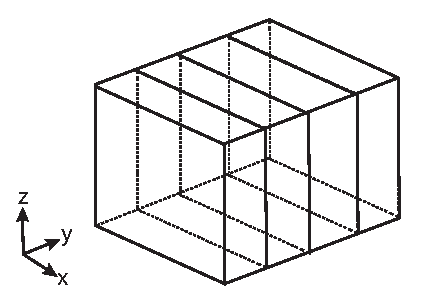
\includegraphics{Figures/2D_slices}
\decoRule
\caption[2D Sclices]{2D slices of the volume.}
\label{fig:2dslices}
\end{figure}
On modern graphics workstations, the complete process of interpolating texture coordinates and reconstructing texture values is incorporated into the scan-conversion process and done completely in hardware. Because texture mapping is such a common application, these routines are well-optimized and highly efficient.
To simulate ray casting using texture mapping, we have to slice the volumetric data set into parallel slices, and the use these slices as texture images to texture-map the projections of the sliced onto the image plane. To composite the slices, we can use the blending operations provided by the OpenGL graphics library. As it happens, one of the standard operators provided is exactly the compositing operator used in ray casting. Since compositing is also fully hardware-assisted, it is also very fast.
\begin{figure}[th]
\centering
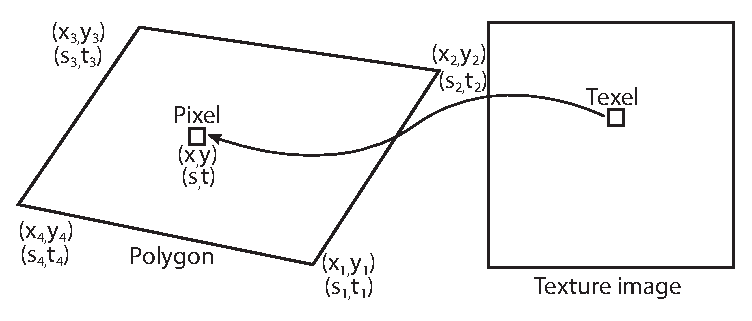
\includegraphics{Figures/2dtexmapping}
\decoRule
\caption[2D texture mapping]{Calculating color and opacity of a pixel inside a texture-mapped polygon.}
\label{fig:2dtexture}
\end{figure}

There are two ways to deal with varying viewpoints.

The first one is to create slice images for the given data set in a pre-processing step and uses different projection matrices to create arbitrary-viewpoint images of these slices. This is fast, since the (expensive) step of slice creation has to be done only once. On the other hand, image quality suffers because the views of all slices will be distorted due to the projection onto the image plane. In the extreme case of the view direction being parallel to the slices, there will be no image at all.

The second way is to create slices which are always orthogonal to the viewing direction. This results in optimal image quality, but it means that the slice stack has to be re-generated for each new image. Furthermore, arbitrary ("oblique") slices through a cuboid are generally not square or rectangular, and can be anything from triangles to hexagons.

\begin{algorithm} \caption{Volume Rendering using 2D Texture Mapping Algorithm} 
\label{alg:tex2dmapping}
\begin{algorithmic}[1]
\Require $N$ the number of slices, $\vec{v} $ the view direction
\State Load the data $\mathcal V(x,y,z) \gets data$ 
\State create the slices $s_i \in \mathcal V$ with each normal $\vec{n_i} \parallel \vec{v}$
\State Turn off the Depth test 
\State Enable the Blending 

\ForEach {$s_i \in \mathcal V $ form back to front}
\State $Texture \gets s_i$
\State create a polygon $p$ corresponding to the slice $s_i$
\State Assign texture coordinates to four corners of the polygon
\State Render and blend the polygon (alpha blending) 
\EndFor

\end{algorithmic}
\end{algorithm}

\paragraph{3D Texture mapping}
To allow interactive generation of view-orthogonal slices, a special hardware technique has been developed. This is a generalization of texture-mapping to three-dimensional textures, appropriately called "3D texturing."
As seen in Figure \ref{fig:2dtexture}, 2D texture-mapping interpolates two additional coordinates (s, t) across a polygon's interior. In 3D texture-mapping, three additional coordinates (s, t, r) are interpolated. To determine a pixel's color and opacity, these three coordinates are used as indices into a three-dimensional image, the 3D texture, see Figure \ref{fig:3dtexture}. To reconstruct texture values, tri-linear interpolation is used.

3D textures allow direct treatment of volumetric data. Instead of generating a set of two-dimensional slices in a pre-processing step, the volumetric data is directly downloaded into the graphics hardware, and is directly used to calculate color and opacity values for each pixel covered by a rendered primitive.

\begin{figure}[th]
\centering
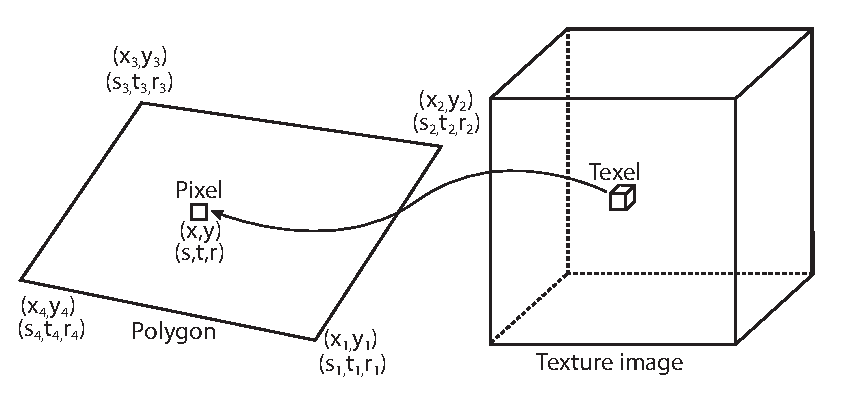
\includegraphics{Figures/3dtexmapping}
\decoRule
\caption[3D texture mapping]{Calculating color and opacity of a pixel inside a texture-mapped polygon using 3D texture.}
\label{fig:3dtexture}
\end{figure}


To generate oblique slices using 3D texturing, one only has to calculate the vertices of the slice, and then to generate the correct 3D texture coordinates for those vertices, see Figure \ref{fig:cubeSlice}. Then these coordinates are passed to the graphics library, and the graphics library will render the projection of the slice onto the image plane, using tri-linear interpolation to reconstruct each pixel's color and opacity values.

\begin{figure}[th]
\centering
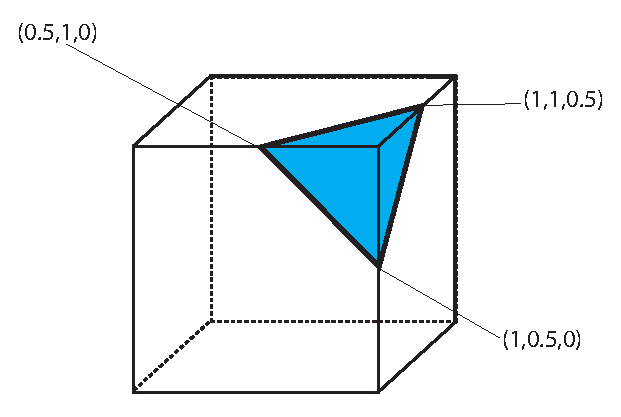
\includegraphics{Figures/cubeSlice}
\decoRule
\caption[3D Cube slice]{Calculating vertex coordinates and texture coordinates for an oblique slice. In this figure, the vertex and texture coordinates are identical.}
\label{fig:cubeSlice}
\end{figure}

\subsubsection{Raycasting}
Volume raycasting computes a 2D image from the 3D volumetric data set.The basic goal of ray casting is to allow the best use of the three-dimensional data and not attempt to impose any geometric structure on it. It solves one of the most important limitations of surface extraction techniques, namely the way in which they display a projection of a thin shell in the acquisition space. Surface extraction techniques fail to take into account that, particularly in medical imaging, data may originate from fluid and other materials which may be partially transparent and should be modeled as such. Ray casting doesn't suffer from this limitation. This algorithm can be split in four main steps (see Figure \ref{fig:rayasting}) :
\begin{itemize}

\item \textbf{Ray casting}. For each pixel of the final image, a ray of sight is shot ("cast") through the volume. At this stage it is useful to consider the volume being touched and enclosed within a bounding primitive, a simple geometric object (usually a cuboid) that is used to intersect the ray of sight and the volume.

\item \textbf{Sampling}. Along the part of the ray of sight that lies within the volume, equidistant sampling points or samples are selected. In general, the volume is not aligned with the ray of sight, and sampling points will usually be located in between voxels. Because of that, it is necessary to interpolate the values of the samples from its surrounding voxels (commonly using trilinear interpolation).

\item \textbf{Shading}. For each sampling point, a transfer function retrieves an RGBA material colour and a gradient of illumination values is computed. The gradient represents the orientation of local surfaces within the volume. The samples are then shaded (i.e. coloured and lit) according to their surface orientation and the location of the light source in the scene.

\item \textbf{Compositing}. After all sampling points have been shaded, they are composited along the ray of sight, resulting in the final colour value for the pixel that is currently being processed. The composition is derived directly from the rendering equation and is similar to blending acetate sheets on an overhead projector. It may work back-to-front, i.e. computation starts with the sample farthest from the viewer and ends with the one nearest to the viewer. This work flow direction ensures that masked parts of the volume do not affect the resulting pixel. The front-to-back order could be more computationally efficient since, the residual ray energy is getting down while ray travels away from camera; so, the contribution to the rendering integral is diminishing therefore more aggressive speed/quality compromise may be applied (increasing of distances between samples along ray is one of such speed/quality trade-offs).

\end{itemize}

\begin{figure}[th]
\centering
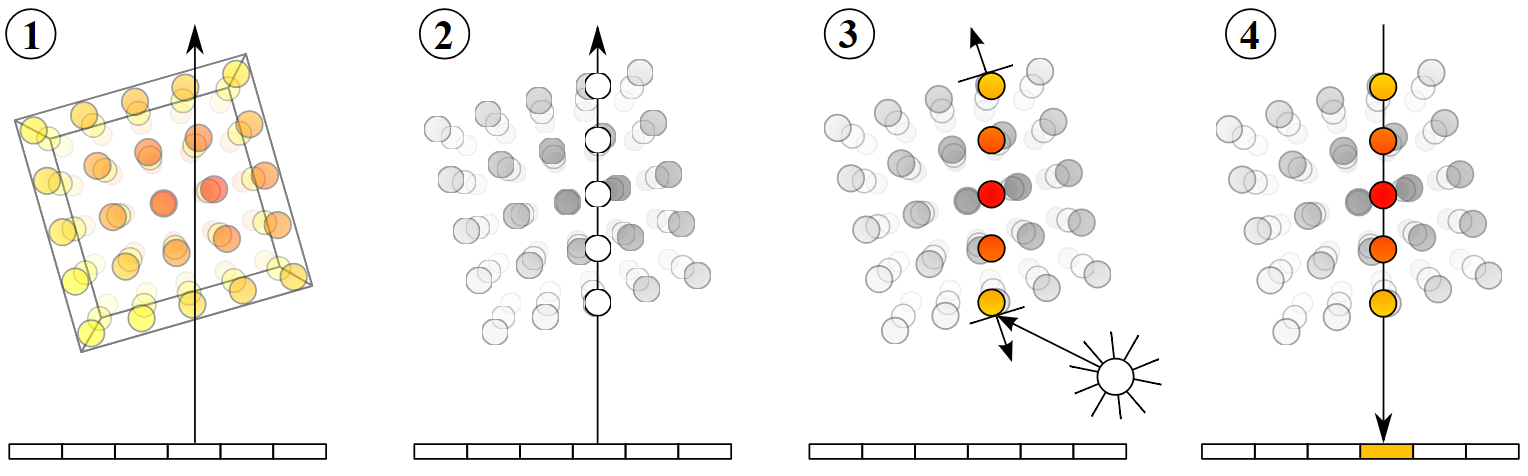
\includegraphics[width=\textwidth]{Figures/raycasting}
\decoRule
\caption[Volume raycasting]{ The four steps of the volume raycasting algorithm  }
\label{fig:rayasting}
\end{figure}

\subsection{Surface-fitting}


\section{Occlusion management strategies}



\subsection{Transfer Function}

A transfer function (TF) maps volumetric data to optical properties
and is part of the traditional visualization pipeline: data acquisition,
processing, visual mapping, and rendering. Volumetric data is
considered to be a scalar function from a three-dimensional spatial
domain with a one-dimensional range (e.g., density, flow magnitude,
etc.). Image generation involves mapping data samples through the
TF, where they are given optical properties such as color and opacity,
and compositing them into the image.
A TF simultaneously defines which parts of the data are essential
to depict and  how to depict these, often small, portions
of the volumetric data. Considering the first step, a TF is a special,
but important, case of a segmentation or classification. With classifi-
cation, certain regions in a three-dimensional domain are identified
to belong to the same material, such as bone, vessel, or soft tissue,
in medical imaging. A plethora of classification and segmentation
algorithms have been developed over the last decades, with semiautomatic
approaches often tailored to specific application scenarios.
Segmentation algorithms can be quite intricate since information
from the three-dimensional spatial domain and the one-dimensional
data range are taken into account. TFs in their basic form are, on the
other hand, restricted to using only the data ranges. In comparison
with general classification algorithms, this characteristic makes a
TF less powerful with respect to identifying relevant parts of the
data. The advantage of a TF is, however, a substantial performance
gain as classification based on the one-dimensional data range reduces
the complexity tremendously. This gain is the result of the
three-dimensional domain being typically two orders of magnitude
larger than the small data range. Histograms are an example of discarding
potentially complex spatial information and aggregating
only the data values to binned-frequency information. In the same
spirit, TFs classify interesting parts of the data by considering data
values alone. The second functionality of a TF deals with specifying
optical properties for portions of the data range previously identified
as being relevant

The transfer functions can be classified according to different criteria. Some of the most important are:

\begin{itemize}
\item \textbf{The dimension: } The one-dimensional TF classifies the scalar data value, $d$, and subsequently maps the material to an optical property for rendering: $ \textbf{q}(d)=\textbf{V}(\textbf{M}(d))$ where $\textbf{M}(.)$ is the material classification function and $\textbf{V}(.)$ is the
visual mapping of the material. One-dimensional TFs are adequate in many cases of simulation data where measurement noise is low or even non-existent where different materials of interest have few overlapping intensity
ranges \cite{4303986}. One-dimensional TFs are often the first tool available in software packages providing volume rendering, as they are relatively easy to comprehend for the novice or occasional user. Practically all production
visualization software, such as ParaView by \cite{paraview},
 VisIt by \cite{Childs:SciDAC2011}, 
or ImageVis3D by {\cite{Fogal2010Tuvok}}, support 1D TF editors.

\begin{figure}[th]
\centering
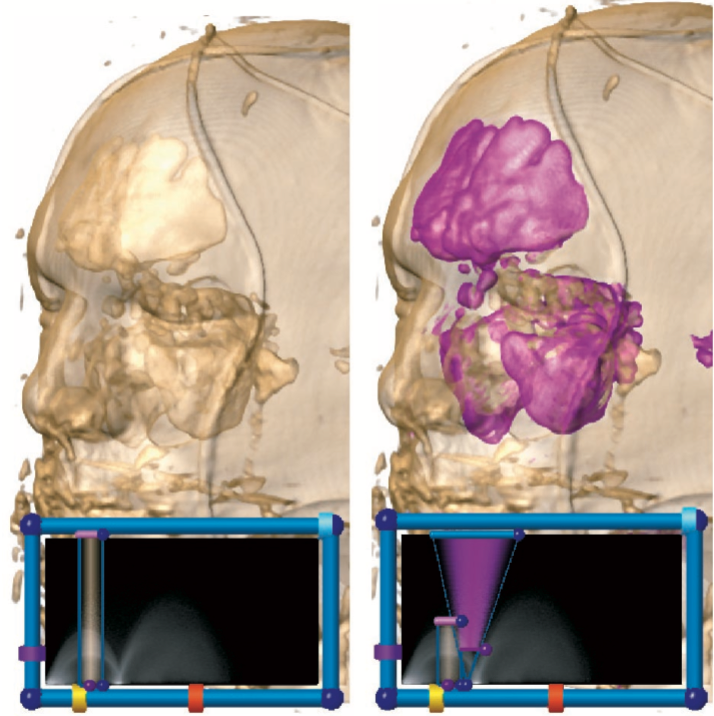
\includegraphics[width=\textwidth]{Figures/2dtf}
\decoRule
\caption[2D transfer Function]{ The two-dimensional TF editor widgets allow the user
to more precisely control the classification power of the 2D TF.
The triangular widget can also be skewed to better fit the desired
classification domain (\cite{1021579}) }
\label{fig:tf2d}
\end{figure}

Multidimensional TFs are used for Multidimensional data. If the user has to manipulate the TF definition directly, moving beyond
2D TFs immediately poses significant challenges in terms of
user interfaces and cognitive comprehension (\cite{1021579}). Much research and
work on Multidimensional TFs is, therefore, related to various forms of automation
and advanced user interfaces. Typical approaches include dimensional reduction, clustering
and grouping, machine learning, and various user interface
approaches such as parallel coordinates by \cite{5742368} or direct slice or volume
view interaction. 

\begin{figure}[th]
\centering
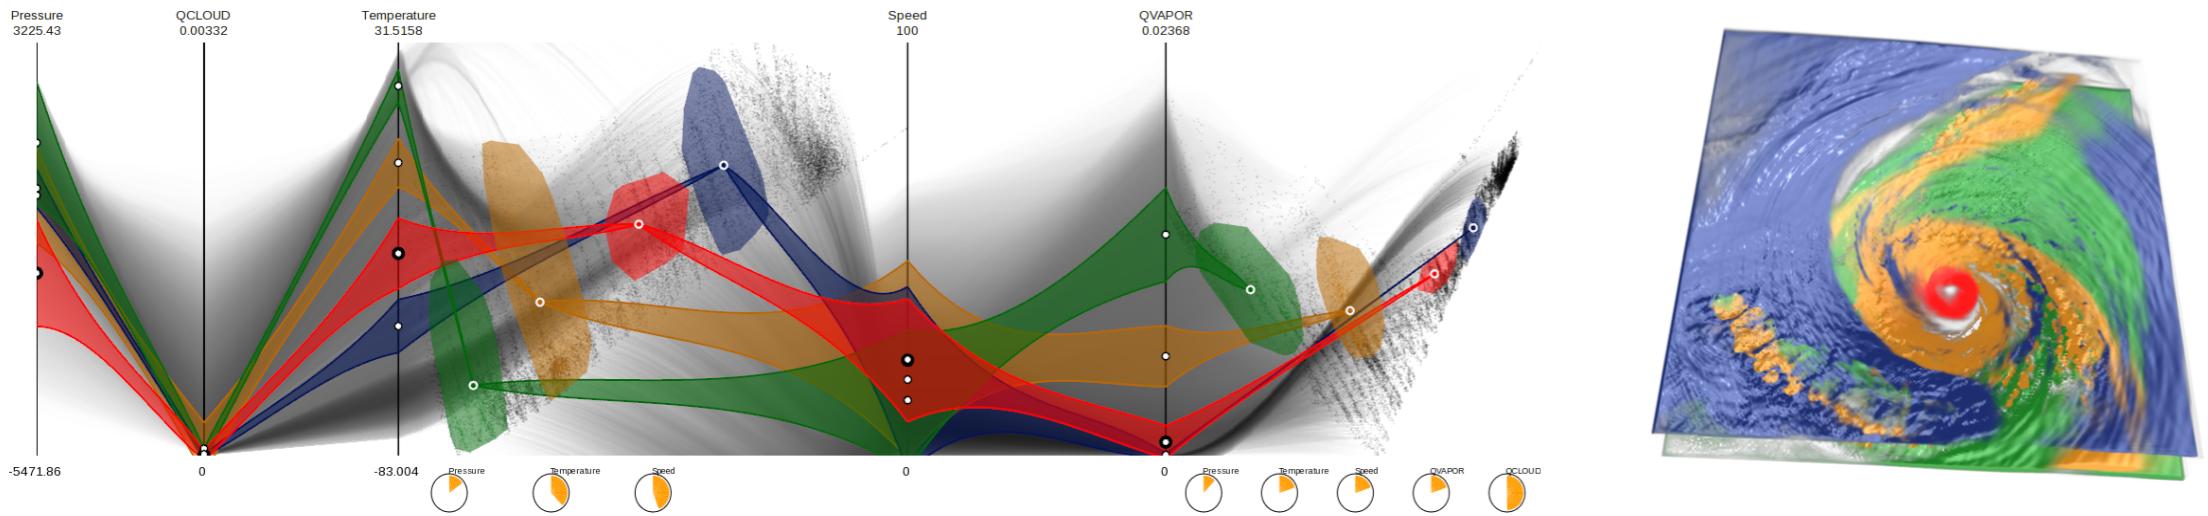
\includegraphics[width=\textwidth]{Figures/mdtf}
\decoRule
\caption[Multidimensional transfer Function]{ Parallel coordinates with embedded multidimensional scale plots for editing multidimensional TFs(\cite{5742368}) }
\label{fig:tfmd}
\end{figure}


\item \textbf{The automation}: The automation includes techniques such as adapting presets, semi-automatic, automatic, and supervised machine learning. Volume rendering has established itself as
a powerful visualization tool in many domains, but the necessary
design of TFs is a time consuming and tedious task. Consequently,
a significant amount of work is dedicated to the automatic and semiautomatic generation of TFs. 

\item \textbf{The aggregated attributes} : Conceptually, the introduction of additional quantities in the TF definition makes it possible to discriminate more parts in a dataset. Histogram clustering helps to reduce the degrees of freedom in designing a TF. As an illustration, \cite{5887324} propose modeling the
histogram space using a Gaussian mixture model. An elliptical TF
is assigned to each Gaussian, and the user interaction is simplified in order to edit the parameters of these ellipsoids.  

\end{itemize}

\subsection{Segmentation}

\subsection{Deformations and Focus + Context}

An interactive lens is a lightweight tool to solve a localized visualization problems by temporarily altering a selected part of the visual representation of the data~\cite{CGF:CGF12871}. Using this lens approach, we propose an interactive volume deformation based on GPU accelerated ray-casting to free a designated target from local occlusion while keeping the global context.

A lens is a parameterizable selection according to which a base visualization is altered. Typically, a lens is added to a visualization to interactively solve a specific localized problem. This property is very interesting with the aim of providing a focus+context solution to occlusion in volume rendering. Lenses can have different geometric properties not only defining their appearance, but also determining the selection, which is the subset of the data where these lenses take effect. The major geometric properties of a lens are shape, position, and size as well as the orientation.
The shape of a lens is usually chosen to fulfill the requirements of the application and is strongly linked to the lens function. Most virtual lenses are circular~\cite{1648236} or are rectangular~\cite{Kincaid:2010:SFA:1907651.1907963} as the real-world ones (magnifying glass, windows). Our lens has also a circular shape in order to remind its magnifying property. Some lenses, such as the  JellyLens~\cite{Pindat:2012:JCA:2380116.2380150} and the smart lenses~\cite{Thiede2008} can adapt their shape automatically according to the data. 
The position and the size parametrization can increase the flexibility of an interactive lens.
Modifying this position or size will set its focus on a different part of the data according to the user's interest. It is possible to update automatically these parameters in order to guide the user toward interesting events in the data~\cite{Tominski:2011:ECU:2336207.2336211}, or adjust the lens position according to predefined paths as the Routelens~\cite{Alvina:2014:RER:2598153.2598200} does. With this mind, our lens updates automatically its properties once a target has been selected. This allows a smooth transition towards an unobstructed and magnified area of interest. 

Lenses for volume visualization face challenges mainly related to spatial selection and occlusion. Wang et al. addressed these issues by proposing the Magic Lens~\cite{1532818}. This Magic Lens renders the obstructions with higher transparency and magnifies volumetric pre-computed features interactively or automatically in a pre-segmented dataset. In addition to interactively magnifying areas and objects of interest, our lens frees them from obstruction and allows local modification of the camera to see the target under other perspectives. Tong et al. proposed the GlyphLens~\cite{7539643} that removes the occluding glyphs by pulling the glyphs aside through the animation, but this tool is only well suited for systems where 3D volumetric dataset are visualized using glyphs. Lenses can create discontinuities between their inner part and the rest of the volume. Deformation can be a solution to this discontinuity issue.   


\begin{figure}[th]
\centering
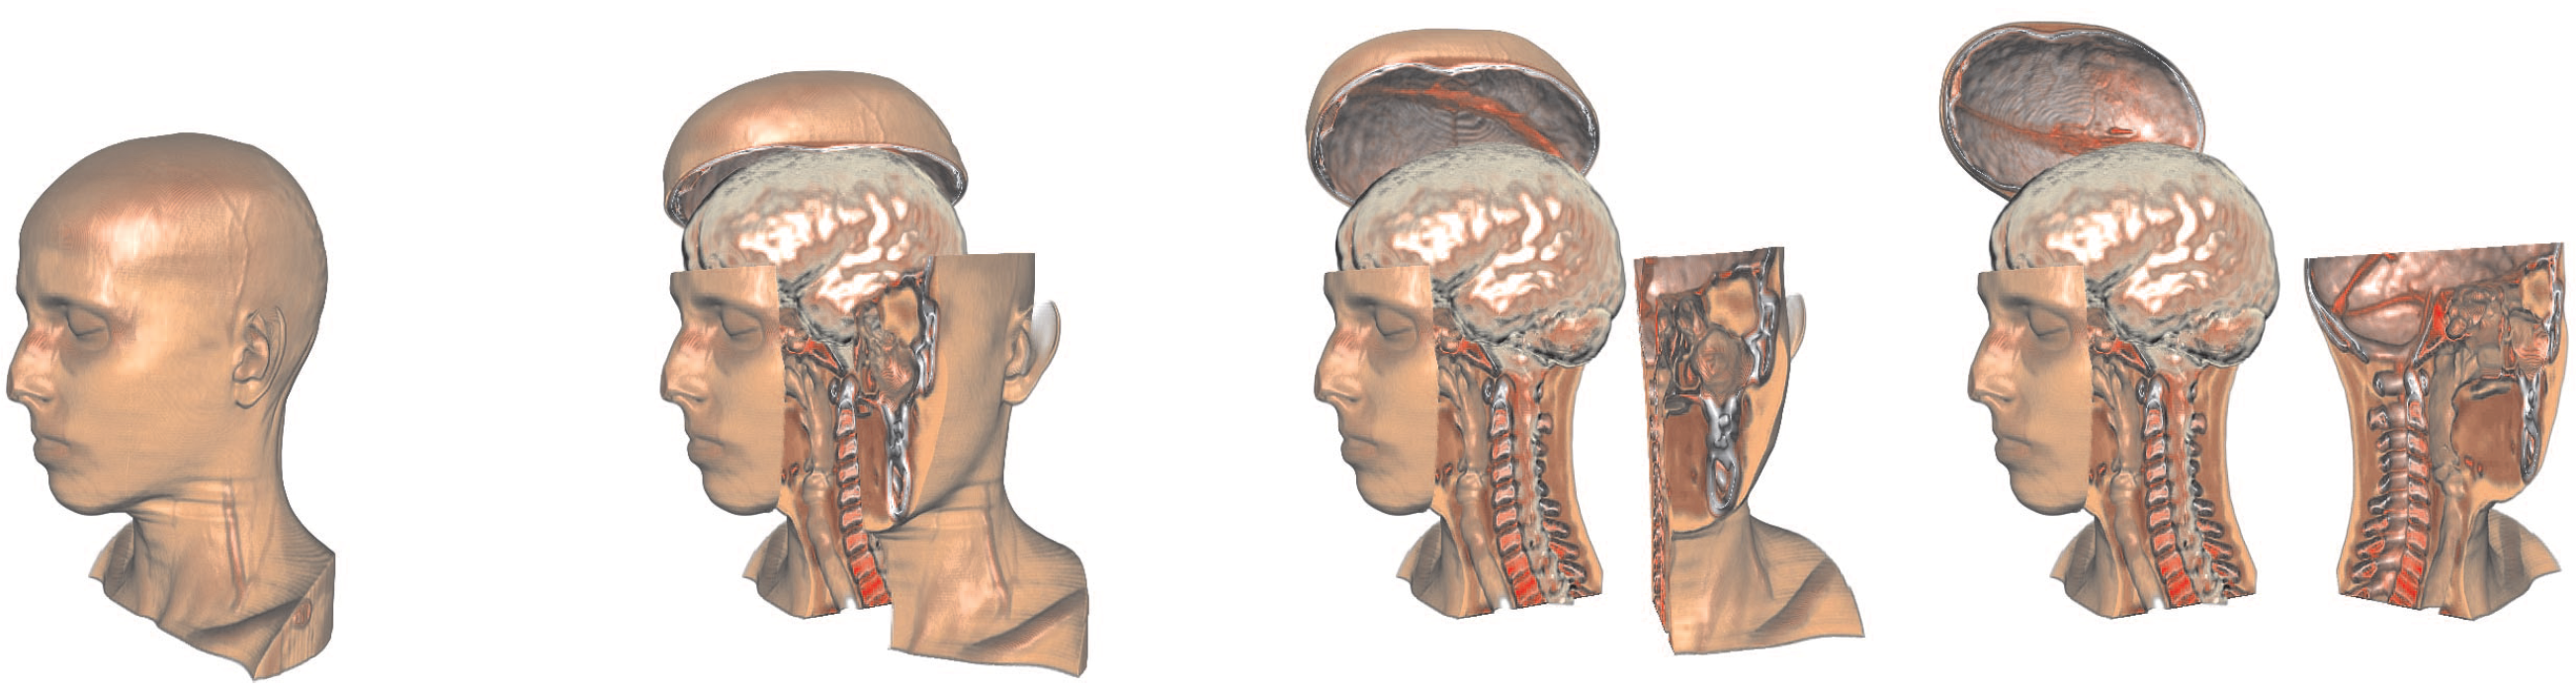
\includegraphics[width=\textwidth]{Figures/explodedview}
\decoRule
\caption[ Interactive exploded-view]{ Interactive exploded-view illustration of a human head with increasing degrees-of-explosion. Two hinge joints are used to constrain part
movement}
\label{fig:exploded}
\end{figure}

Hsu et al. developed a framework that can generate non-linear sampling rays that smoothly project objects in a scene at multiple levels of detail onto a single image~\cite{Hsu:2011:RFM:2070781.2024165}. Such a technique requires a lot of computational time to render a single image from features of interest at different scales.
  Bruckner and  Groller~\cite{4015467} proposed exploded view for volume data by partitioning the volume into several segments \ref{fig:exploded}, while Correa et al. proposed a framework~\cite{Correa:2007:IDD:1313046.1313163} allowing the users to physically or actively manipulate the geometry of a data object. McGuffin et al.~\cite{1250400} performed deformations using peeling to see hidden parts of the data. However, these techniques have the disadvantage of removing potentially important surrounding contextual information while trying to solve the local occlusion. 
 
 
Deformations can reveal predefined features in the dataset by taking into account the precomputed segmentation. Tong et al. proposed a deforming Lens which moves streamlines to observe the inner part of streamline bundles~\cite{7332955}. Some studies performed deformations using surgical metaphors ~\cite{4069230,Correa:2006:FAV:1187627.1187827} to see hidden parts of the volume, but they do not offer tools for local manipulation of the point of view which allows perceiving a target under a different perspective while keeping the global context.


\section{Volume rendering in Virtual Reality and Augmented Reality}

\subsection{ Remote volume rendering}

Volumetric data exploration with direct volume rendering technique is of great help to visually extract relevant structures in many fields of science: medical imaging ~\cite{ljung_full_2006}, astrophysics and more recently in baggage inspection. To leverage this knowledge extraction, many techniques have been developed. 

In this section, we detail existing ones with volume visualization, transfer function, direct voxel manipulation, and focus plus context interaction.
Volume visualization can be done with geometric rendering system which transforms the data into a set of polygons representing an iso-surface. The contour tree algorithm ~\cite{carr_computing_2000} and other alternatives such as branch decomposition ~\cite{pascucci_multi-resolution_2004} are usually used to find these iso-surfaces. According to H. Guo ~\cite{guo_local_2013}, contour trees algorithms are vulnerable to noises, which can be problematic in baggage inspections since dense materials (e.g. iron) cause noises by reflecting the X-rays. For this reason we used the volume rendering technique; Chen et al. provide a review of existing techniques ~\cite{chen_3-d_2000}.
In order to investigate volumetric dataset, one can use the Transfer Function (TF). In practice, it maps the voxel density with a specific color (including its transparency). Transfer function can be 1D, 2D or nD and are of great help to isolate structures of interest in volumetric data ~\cite{kniss_multidimensional_2002}. Thanks to the color blending process, suitable transfer function can also reveal iso surface or hide density to improve the volumetric data visualization. The setup of this transfer function remains complex, but some automatic systems provide solution thanks to data analysis ~\cite{correa_size-based_2008} ~\cite{sereda_visualization_2006} ~\cite{patel_moment_2009} or user interactions ~\cite{guo_wysiwyg_2011}. Since our users have a limited knowledge on volume rendering, we developed new interaction techniques with sufficient abstraction level regarding technical constraints. These techniques will be detailed in this paper. As an example, we investigated predefined transfer functions with smooth transitions when changing their setup to reduce disruptive animation effects ~\cite{tversky_animation:_2002}.
Since graphic card power never stops to improve, new techniques allow the direct manipulation of the voxels which composes the volume to be displayed. Color tunneling introduced a set of interactions (lock, Brush, Dig) to explore 2D and 3D dataset composed of pixels of voxels ~\cite{hurter_interactive_2014} with point based rendering techniques ~\cite{sainz_point-based_2004} . Histomage also provides direct manipulation of pixels thanks to a histogram which can be used as a new selection and pixel modification tool ~\cite{chevalier_histomages:_2012}. Other interactive systems investigated pixel exploration with a lens as a focus plus context technique ~\cite{elmqvist_color_2011} ~\cite{hurter_moleview:_2011}. Our work provides additional interaction techniques with pixel based techniques ~\cite{hurter_interactive_2014} to address occlusion issues, focus and context awareness, reversibility of the actions, and continuity.  